\documentclass[12pt]{article}
\usepackage[margin=1in]{geometry}
\usepackage{amsmath,amssymb,mathtools}
\usepackage{enumitem}
\usepackage{bm}
\usepackage{hyperref}
\usepackage{fancyhdr}
\usepackage{draftwatermark}
\usepackage{xcolor}
\usepackage{pgfplots}
\pgfplotsset{compat=newest}

%------------- TITLE AND METADATA -------------

\newcommand{\CourseCode}{HE2001 }
\newcommand{\CourseName}{Microeconomics II}
\newcommand{\DocType}{Tutorial 4}

\title{
\CourseCode \CourseName \\[0.3em]
\large \DocType
}
\author{
  Academic Year 2025/2026, Semester 2 \\[0.25em]
  \textit{Quantitative Research Society @NTU}
}
\date{\today}

%----------------------------------------------

%------------- HEADER & FOOTER (for page 2 onward) -------------
\fancypagestyle{main}{
  \fancyhf{}
  \fancyhead[L]{\CourseCode \CourseName}
  \fancyhead[R]{\href{[https://qrsntu.org](https://qrsntu.org)}{QRS@NTU}}
  \fancyfoot[C]{\thepage}
  \renewcommand{\headrulewidth}{0.4pt}
  \renewcommand{\footrulewidth}{0pt}
}

%------------- SIMPLE FOOTER (page 1 only) -------------
\fancypagestyle{plainfirst}{
  \fancyhf{}
  \renewcommand{\headrulewidth}{0pt}
  \renewcommand{\footrulewidth}{0pt}
  \fancyfoot[C]{\scriptsize\textcolor{gray}{\textit{For academic reference only. This document is provided for educational purposes and does not constitute an official question paper, answer key, or any formally authorised academic material. Its content is not guaranteed to be complete or accurate.}}}
}

%------------- WATERMARK -------------
\SetWatermarkText{Unofficial — QRS@NTU — qrsntu.org}
\SetWatermarkScale{1}
\SetWatermarkLightness{0.99}
%------------------------------------

%------------- SHORTCUTS -------------
\newcommand{\R}{\mathbb{R}}
\newcommand{\Rp}{\mathbb{R}_+}
\newcommand{\dotp}{\cdot}
%------------------------------------

\begin{document}

%------------- COVER PAGE -------------
\maketitle
\thispagestyle{plainfirst}
\pagestyle{main}
\bigskip

%====================================================
% OVERVIEW
%====================================================
\begin{center}
  \rule{0.8\textwidth}{0.4pt}\\[4pt]
  \textbf{Overview}\\[2pt]
  \rule{0.8\textwidth}{0.4pt}
\end{center}

\noindent
This tutorial covers:
\begin{itemize}[leftmargin=*]
  \item discounted utility with log preferences and intertemporal demand;
  \item comparative statics in the discount factor \(\delta\) and interest rate \(r\);
  \item borrowing vs saving with different interest rates (kinked intertemporal budget sets);
  \item ranking assets by present value and identifying arbitrage;
  \item no-arbitrage pricing and comparative statics of price ratios.
\end{itemize}

\bigskip

%====================================================
% PART 1
%====================================================
\newpage
\section{Discounted Utility}

Suppose utility is \(U(x_0,x_1)=u(x_0)+\delta u(x_1)\) where \(u(x)=\ln(x)\).
Recall that \(u'(x)=\frac{1}{x}\).
Suppose the consumer buys consumption to maximize utility subject to a budget constraint
\[
p_0x_0+p_1x_1=m.
\]
Thus, when the consumer maximizes utility his demand will satisfy
\[
\frac{u'(x_0)}{\delta u'(x_1)}=\frac{p_0}{p_1}.
\]

\subsection{Log utility demand}
Find the demand function: \(x(p,m)=(x_0(p,m),x_1(p,m))\). So, \(x_k(p,m)\) should tell you
how much the consumer demands of good \(k\) when price is \(p\) and expenditure level is
\(m\).

\subsection*{Solution}
\subsubsection*{Method 1: Lagrangian and FOCs}
Maximise
\[
\ln x_0+\delta \ln x_1
\quad\text{s.t.}\quad
p_0x_0+p_1x_1=m,\qquad x_0>0,\ x_1>0.
\]
Lagrangian:
\[
\mathcal{L}=\ln x_0+\delta \ln x_1+\lambda(m-p_0x_0-p_1x_1).
\]
FOCs:
\[
\frac{1}{x_0}-\lambda p_0=0,\qquad
\frac{\delta}{x_1}-\lambda p_1=0,\qquad
p_0x_0+p_1x_1=m.
\]
From the first two,
\[
\lambda=\frac{1}{p_0x_0}=\frac{\delta}{p_1x_1}\quad\Rightarrow\quad p_1x_1=\delta p_0x_0.
\]
Substitute into the budget:
\[
m=p_0x_0+p_1x_1=p_0x_0+\delta p_0x_0=(1+\delta)p_0x_0
\Rightarrow
x_0(p,m)=\frac{m}{(1+\delta)p_0}.
\]
Then
\[
x_1(p,m)=\frac{\delta p_0}{p_1}x_0=\frac{\delta p_0}{p_1}\cdot \frac{m}{(1+\delta)p_0}
=\frac{\delta m}{(1+\delta)p_1}.
\]
\[
\boxed{\;x_0(p,m)=\frac{m}{(1+\delta)p_0},\qquad x_1(p,m)=\frac{\delta m}{(1+\delta)p_1}\;}
\]

\subsubsection*{Method 2: Spending-share (ratio) method}
The FOC condition given implies
\[
\frac{(1/x_0)}{\delta(1/x_1)}=\frac{p_0}{p_1}
\quad\Rightarrow\quad
\frac{x_1}{\delta x_0}=\frac{p_0}{p_1}
\quad\Rightarrow\quad
p_1x_1=\delta p_0x_0.
\]
Let \(S_0=p_0x_0\) and \(S_1=p_1x_1\). Then \(S_1=\delta S_0\) and \(S_0+S_1=m\), so
\[
(1+\delta)S_0=m \Rightarrow S_0=\frac{m}{1+\delta},\quad S_1=\frac{\delta m}{1+\delta}.
\]
Hence
\[
x_0=\frac{S_0}{p_0}=\frac{m}{(1+\delta)p_0},\qquad
x_1=\frac{S_1}{p_1}=\frac{\delta m}{(1+\delta)p_1}.
\]
\[
\boxed{\;x_0(p,m)=\frac{m}{(1+\delta)p_0},\qquad x_1(p,m)=\frac{\delta m}{(1+\delta)p_1}\;}
\]

\subsection{Effect of \texorpdfstring{\(\delta\)}{delta} on \(x_0\)}
What happens to the demand for good 0 as \(\delta\) increases?

\subsection*{Solution}
\subsubsection*{Method 1: Differentiate the closed-form demand}
From the demand,
\[
x_0(\delta)=\frac{m}{(1+\delta)p_0}
\quad\Rightarrow\quad
\frac{\partial x_0}{\partial \delta}
=-\frac{m}{p_0}\cdot\frac{1}{(1+\delta)^2}<0.
\]
\[
\boxed{\;\text{As }\delta\text{ increases, }x_0\text{ decreases.}\;}
\]

\subsubsection*{Method 2: Expenditure share argument}
The spending ratio satisfies
\[
\frac{p_1x_1}{p_0x_0}=\delta.
\]
As \(\delta\) rises, the consumer allocates a larger share to good 1 relative to good 0, holding total expenditure \(m\) fixed. Since \(p_0x_0=m/(1+\delta)\) is decreasing in \(\delta\), \(x_0\) decreases.
\[
\boxed{\;\text{As }\delta\uparrow,\ \text{the consumer shifts spending toward period 1, so }x_0\downarrow.\;}
\]

\subsection{Effect of \(r\) with prices \(p=(1,\frac{1}{1+r})\)}
Suppose prices take the form \(p=\bigl(1,\frac{1}{1+r}\bigr)\). What happens to the demand for good 0 as
\(r\) increases (equivalently what happens to the demand for good 0 when \(p_1\) decreases)?

\subsection*{Solution}
\subsubsection*{Method 1: Plug into \(x_0(p,m)\) with fixed \(m\)}
The demand is
\[
x_0(p,m)=\frac{m}{(1+\delta)p_0}.
\]
Here \(p_0=1\), so
\[
x_0=\frac{m}{1+\delta},
\]
which does not depend on \(p_1=\frac{1}{1+r}\) (and hence does not depend on \(r\)) when \(m\) is fixed.
\[
\boxed{\;\text{Holding }m\text{ fixed, }x_0\text{ does not change as }r\text{ increases.}\;}
\]

\subsubsection*{Method 2: Eliminate \(p_1\) using the FOC}
From the FOC, \(p_1x_1=\delta p_0x_0\). Substitute into the budget:
\[
m=p_0x_0+p_1x_1=p_0x_0+\delta p_0x_0=(1+\delta)p_0x_0
\Rightarrow
x_0=\frac{m}{(1+\delta)p_0},
\]
which does not involve \(p_1\) at all. Therefore changing \(r\) (changing \(p_1\)) has no effect on \(x_0\) if \(m\) is fixed.
\[
\boxed{\;\text{Holding }m\text{ fixed, }x_0\text{ is independent of }r.\;}
\]

\subsection{Present value of income}
Suppose the consumer has income \((y_0,y_1)=(0,100)\) and the interest rate is \(r\). What
is the present value of this income?

\subsection*{Solution}
\subsubsection*{Method 1: Discount the period-1 income}
\[
PV=y_0+\frac{y_1}{1+r}=0+\frac{100}{1+r}.
\]
\[
\boxed{\;PV=\frac{100}{1+r}\;}
\]

\subsubsection*{Method 2: Replication by saving/borrowing}
Find \(M\) such that saving \(M\) at \(t=0\) yields \(100\) at \(t=1\):
\[
M(1+r)=100\Rightarrow M=\frac{100}{1+r}.
\]
\[
\boxed{\;PV=\frac{100}{1+r}\;}
\]

\subsection{Effect of \(r\) when income is \((0,100)\)}
Continue to assume the consumer has income \((0,100)\). What happens to the consumer’s
demand for good 0 as \(r\) increases (note that increasing \(r\) changes the present value of
the income stream)?

\subsection*{Solution}
\subsubsection*{Method 1: Treat expenditure as present value \(m(r)\)}
With income \((0,100)\), the present value is
\[
m(r)=\frac{100}{1+r}.
\]
With prices \(p=\bigl(1,\frac{1}{1+r}\bigr)\), we have \(p_0=1\), so
\[
x_0(r)=\frac{m(r)}{1+\delta}=\frac{1}{1+\delta}\cdot\frac{100}{1+r}.
\]
Since \(\frac{100}{1+r}\) decreases in \(r\), \(x_0(r)\) decreases in \(r\).
\[
\boxed{\;\text{As }r\text{ increases, }x_0\text{ decreases.}\;}
\]

\subsubsection*{Method 2: Monotonicity via PV}
The PV of the income stream is strictly decreasing:
\[
PV(r)=\frac{100}{1+r}\downarrow \text{ as }r\uparrow.
\]
But \(x_0=\frac{m}{1+\delta}\) when \(p_0=1\). Hence \(x_0\) moves one-for-one with \(m=PV(r)\), so \(x_0\) decreases.
\[
\boxed{\;\text{As }r\uparrow,\ PV\downarrow\Rightarrow x_0\downarrow.\;}
\]

\subsection{Numerical demand with given \(\delta\) and \(r\)}
Assume the consumer has income \((0,24)\). Suppose that \(\delta=\frac{1}{2}\) and that the interest
rate is \(r=1\). How much will be demanded of good 0 and 1?

\subsection*{Solution}
\subsubsection*{Method 1: Compute PV, then apply demand}
Present value:
\[
m=\frac{24}{1+r}=\frac{24}{2}=12.
\]
Prices: \(p_0=1\), \(p_1=\frac{1}{1+r}=\frac12\). With \(\delta=\frac12\),
\[
x_0=\frac{m}{(1+\delta)p_0}=\frac{12}{(1+\frac12)\cdot 1}=\frac{12}{3/2}=8,
\]
\[
x_1=\frac{\delta m}{(1+\delta)p_1}
=\frac{\frac12\cdot 12}{\frac32\cdot \frac12}
=\frac{6}{3/4}=8.
\]
\[
\boxed{\;x_0=8,\qquad x_1=8\;}
\]

\subsubsection*{Method 2: Use FOC ratio and budget directly}
FOC gives \(p_1x_1=\delta p_0x_0\). Here \(\delta=\frac12\), \(p_0=1\), \(p_1=\frac12\):
\[
\frac12 x_1=\frac12 x_0\Rightarrow x_1=x_0.
\]
Budget uses PV \(m=12\):
\[
x_0+\frac12 x_1=12.
\]
Substitute \(x_1=x_0\):
\[
x_0+\frac12 x_0=\frac32 x_0=12\Rightarrow x_0=8\Rightarrow x_1=8.
\]
\[
\boxed{\;x_0=8,\qquad x_1=8\;}
\]

%====================================================
% PART 2
%====================================================
\newpage
\section{Interest rates}

Suppose you can borrow at interest rate \(r_b\) and save at rate \(r_s\).
You are endowed with \(y=(1,1)\).

\subsection{Budget line with borrowing expensive}
Draw the budget line when \(2=r_b>r_s=1\) (note that the budget line is not in-fact a
straight line).

\subsection*{Solution}
\begin{figure}[htpb]
    \centering
    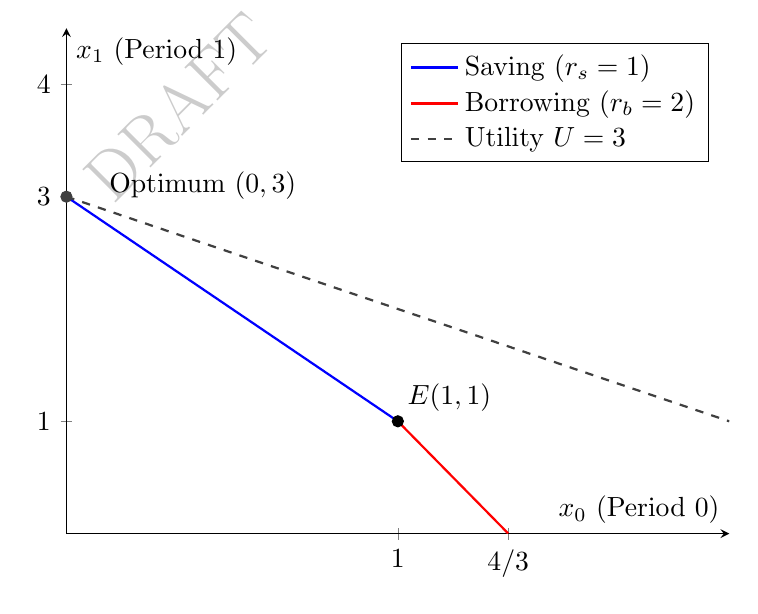
\begin{tikzpicture}
        \begin{axis}[
            axis lines = center,
            xlabel = {$x_0$ (Period 0)},
            ylabel = {$x_1$ (Period 1)},
            xmin = 0, xmax = 2,
            ymin = 0, ymax = 4.5,
            xtick = {1, 1.333},
            xticklabels = {1, $4/3$},
            ytick = {1, 3, 4},
            legend pos = north east,
            legend cell align = {left},
            grid = none,
            width = 10cm,
            height = 8cm
        ]
        
        % Saving Region
        \addplot [domain=0:1, thick, blue] {3 - 2*x};
        \addlegendentry{Saving ($r_s=1$)}
        
        % Borrowing Region
        \addplot [domain=1:1.333, thick, red] {4 - 3*x};
        \addlegendentry{Borrowing ($r_b=2$)}
        
        % Highest Utility Indifference Curve U=3
        \addplot [domain=0:2, dashed, darkgray, thick] {3 - x};
        \addlegendentry{Utility $U=3$}
        
        % Endowment Point
        \addplot[mark=*, black] coordinates {(1,1)};
        \node[above right] at (axis cs:1,1) {$E(1,1)$};
        
        % Optimum Point
        \addplot[mark=*, darkgray] coordinates {(0,3)};
        \node[right] at (axis cs:0.1, 3.1) {Optimum $(0,3)$};
        
        \end{axis}
    \end{tikzpicture}
    \caption{Budget frontier and optimal choice with expensive borrowing ($r_b=2, r_s=1$).}
    \label{fig:borrow_expensive}
\end{figure}

Let \(x_0\) be period-0 consumption and \(x_1\) period-1 consumption. Endowment is \((1,1)\).

\subsubsection*{Method 1: Derive saving and borrowing pieces}
\paragraph{Saving region \((x_0\le 1)\).}
Saving \(s=1-x_0\ge 0\) yields \((1+r_s)s\) next period:
\[
x_1=1+(1+r_s)(1-x_0).
\]
With \(r_s=1\):
\[
x_1=1+2(1-x_0)=3-2x_0,\qquad (0\le x_0\le 1).
\]

\paragraph{Borrowing region \((x_0\ge 1)\).}
Borrowing \(b=x_0-1\ge 0\) requires repayment \((1+r_b)b\):
\[
x_1=1-(1+r_b)(x_0-1).
\]
With \(r_b=2\):
\[
x_1=1-3(x_0-1)=4-3x_0,\qquad (1\le x_0\le 4/3).
\]
\[
\boxed{\;\text{Budget frontier: }x_1=3-2x_0\ (x_0\le 1),\ \ x_1=4-3x_0\ (x_0\ge 1).\;}
\]

\subsubsection*{Method 2: Slopes through the endowment point}
The frontier passes through \((1,1)\). Slopes are \(-\,(1+r_s)=-2\) when saving and \(-\,(1+r_b)=-3\) when borrowing. Hence:
\[
x_1-1=-2(x_0-1)\Rightarrow x_1=3-2x_0\ (x_0\le 1),
\]
\[
x_1-1=-3(x_0-1)\Rightarrow x_1=4-3x_0\ (x_0\ge 1).
\]
\[
\boxed{\;\text{Same piecewise budget frontier.}\;}
\]

\subsection{Budget line with saving more attractive}
Draw the budget line when \(r_s'=2\) and \(r_b'=1\).

\subsection*{Solution}
\subsubsection*{Method 1: Piecewise derivation}

\begin{figure}[htpb]
    \centering
    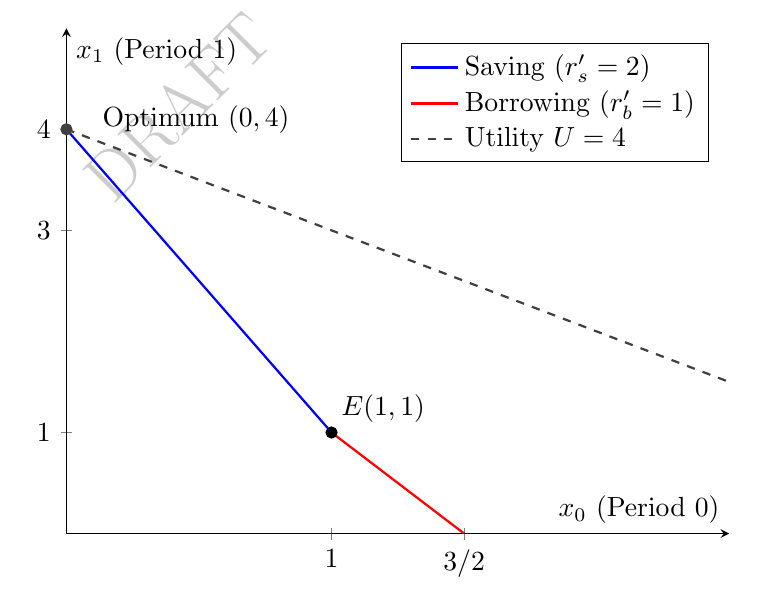
\begin{tikzpicture}
        \begin{axis}[
            axis lines = center,
            xlabel = {$x_0$ (Period 0)},
            ylabel = {$x_1$ (Period 1)},
            xmin = 0, xmax = 2.5,
            ymin = 0, ymax = 5,
            xtick = {1, 1.5},
            xticklabels = {1, $3/2$},
            ytick = {1, 3, 4},
            legend pos = north east,
            legend cell align = {left},
            grid = none,
            width = 10cm,
            height = 8cm
        ]
        
        % Saving Region
        \addplot [domain=0:1, thick, blue] {4 - 3*x};
        \addlegendentry{Saving ($r_s'=2$)}
        
        % Borrowing Region
        \addplot [domain=1:1.5, thick, red] {3 - 2*x};
        \addlegendentry{Borrowing ($r_b'=1$)}
        
        % Highest Utility Indifference Curve U=4
        \addplot [domain=0:2.5, dashed, darkgray, thick] {4 - x};
        \addlegendentry{Utility $U=4$}
        
        % Endowment Point
        \addplot[mark=*, black] coordinates {(1,1)};
        \node[above right] at (axis cs:1,1) {$E(1,1)$};
        
        % Optimum Point
        \addplot[mark=*, darkgray] coordinates {(0,4)};
        \node[right] at (axis cs:0.1, 4.1) {Optimum $(0,4)$};
        
        \end{axis}
    \end{tikzpicture}
    \caption{Budget frontier and optimal choice with attractive saving ($r_b'=1, r_s'=2$).}
    \label{fig:save_attractive}
\end{figure}

\paragraph{Saving \((x_0\le 1)\).}
\[
x_1=1+(1+r_s')(1-x_0)=1+3(1-x_0)=4-3x_0.
\]
\paragraph{Borrowing \((x_0\ge 1)\).}
\[
x_1=1-(1+r_b')(x_0-1)=1-2(x_0-1)=3-2x_0.
\]
\[
\boxed{\;\text{Budget frontier: }x_1=4-3x_0\ (x_0\le 1),\ \ x_1=3-2x_0\ (x_0\ge 1).\;}
\]

\subsubsection*{Method 2: Slopes through \((1,1)\)}
Saving slope is \(-\,(1+r_s')=-3\) and borrowing slope is \(-\,(1+r_b')=-2\). Through \((1,1)\):
\[
x_1-1=-3(x_0-1)\Rightarrow x_1=4-3x_0,\quad
x_1-1=-2(x_0-1)\Rightarrow x_1=3-2x_0.
\]
\[
\boxed{\;\text{Same piecewise budget frontier.}\;}
\]

\subsection{Preference over interest-rate regimes with linear utility}
Suppose the consumer has \(U(x_0,x_1)=x_0+x_1\) (note discount factor \(\delta=1\)). Does the
consumer prefer interest rates \((r_b,r_s)\) or \((r_b',r_s')\)? That is, under which pair of interest
rates can the consumer buy a bundle with greater utility?

\subsection*{Solution}
\subsubsection*{Method 1: Evaluate utility at key corners}
With linear utility and positive coefficients, the optimum occurs at an extreme point.

\paragraph{Regime \((r_b,r_s)=(2,1)\).}
Corners: \((0,3)\), \((1,1)\), \((4/3,0)\).
\[
U(0,3)=3,\quad U(1,1)=2,\quad U(4/3,0)=4/3.
\]
Maximum \(=3\).

\paragraph{Regime \((r_b',r_s')=(1,2)\).}
Corners: \((0,4)\), \((1,1)\), \((3/2,0)\).
\[
U(0,4)=4,\quad U(1,1)=2,\quad U(3/2,0)=3/2.
\]
Maximum \(=4\).
\[
\boxed{\;\text{The consumer prefers }(r_b',r_s')\text{ since }4>3.\;}
\]

\subsubsection*{Method 2: Maximise along each piece (monotonicity)}
For \((2,1)\): on saving piece \(x_1=3-2x_0\), \(U=3-x_0\) maximised at \(x_0=0\Rightarrow 3\); borrowing piece yields at most \(2\).  
For \((1,2)\): on saving piece \(x_1=4-3x_0\), \(U=4-2x_0\) maximised at \(x_0=0\Rightarrow 4\).  
Thus \((1,2)\) dominates.
\[
\boxed{\;\text{Prefer }(r_b',r_s').\;}
\]

%====================================================
% PART 3
%====================================================
\newpage
\section{Comparing assets}

Consider three assets: \(y^{A}=(1,0,0)\), \(y^{B}=(0,3,0)\), and \(y^{C}=(0,0,4)\).

\subsection{Best asset by present value}
For what interest rates \(r\) is \(A\) the best? What about \(B\) and \(C\)? To answer consider the
present values.

\subsection*{Solution}
Let
\[
PV(y;r)=y_0+\frac{y_1}{1+r}+\frac{y_2}{(1+r)^2}.
\]
Then
\[
PV_A=1,\qquad PV_B=\frac{3}{1+r},\qquad PV_C=\frac{4}{(1+r)^2}.
\]

\subsubsection*{Method 1: Pairwise comparisons}
\(B\) vs \(C\):
\[
\frac{3}{1+r}\ge \frac{4}{(1+r)^2}
\iff 3(1+r)\ge 4
\iff r\ge \frac{1}{3}.
\]
\(A\) vs \(B\):
\[
1\ge \frac{3}{1+r}\iff 1+r\ge 3\iff r\ge 2.
\]
\(A\) vs \(C\):
\[
1\ge \frac{4}{(1+r)^2}\iff (1+r)^2\ge 4\iff r\ge 1.
\]
Thus:
\[
\boxed{\;\text{\(C\) best if }r<\frac13;\quad \text{\(B\) best if }\frac13\le r\le 2;\quad \text{\(A\) best if }r>2.\;}
\]

\subsubsection*{Method 2: Cutoff reasoning}
Solve equalities:
\[
PV_B=PV_C \Rightarrow r=\frac13,\qquad PV_A=PV_B\Rightarrow r=2.
\]
As \(r\to 0\), \(PV_C\to 4\) is largest; as \(r\to\infty\), \(PV_A=1\) dominates. Hence the ordering must be \(C\) then \(B\) then \(A\) across the two cutoffs.
\[
\boxed{\;\text{Same cutoff partition: }r=\frac13,\ 2.\;}
\]

\newpage
\subsection{Effect of endowment \((2,0,0)\) on rankings}
Answer the same question when you are endowed with \((2,0,0)\). That is, if you take
asset \(y^{A}\) then you get \((2,0,0)+y^{A}\) and so forth.

\subsection*{Solution}
\subsubsection*{Method 1: Additivity of present value}
\[
PV((2,0,0)+y;r)=PV(2,0,0;r)+PV(y;r)=2+PV(y;r).
\]
Adding the same constant \(2\) to all options does not change rankings.
\[
\boxed{\;\text{The ranking (and cutoffs) are unchanged.}\;}
\]

\subsubsection*{Method 2: Pairwise comparisons cancel the endowment}
For any two assets \(y,\tilde y\),
\[
PV(e+y;r)\ge PV(e+\tilde y;r)\iff PV(y;r)\ge PV(\tilde y;r).
\]
Thus endowment does not affect which asset is best.
\[
\boxed{\;\text{Same ranking as in Question 3.1.}\;}
\]

\subsection{Arbitrage with overpriced asset \(B\)}
Now, assume that you have no money \((0,0,0)\) and asset \(B\) costs
\[
\frac{4}{1+r}.
\]
Can you find an arbitrage opportunity?

\subsection*{Solution}
\subsubsection*{Method 1: Compare to no-arbitrage PV and construct a strategy}
Asset \(B\) pays \((0,3,0)\), so its no-arbitrage price is
\[
PV_B=\frac{3}{1+r}.
\]
Given price \(p_B=\frac{4}{1+r}>\frac{3}{1+r}\), \(B\) is overpriced.

Arbitrage:
\begin{itemize}[leftmargin=*]
\item At \(t=0\): short-sell 1 unit of \(B\), receive \(\frac{4}{1+r}\). Invest at rate \(r\).
\item At \(t=1\): investment becomes \((1+r)\frac{4}{1+r}=4\). Pay the short obligation payoff \(3\). Keep \(1\) risk-free.
\item No further payoffs.
\end{itemize}
\[
\boxed{\;\text{Yes: short }B\text{ and invest; sure profit }1\text{ at }t=1.\;}
\]

\subsection{Comparative statics of price ratio \(p_A/p_C\)}
Let \(p_A\) and \(p_C\) be the prices of asset \(A\) and \(C\) in period 0. What happens to the ratio
\[
\frac{p_A}{p_C}
\]
as \(r\) increases (assume \(p_A\) and \(p_C\) are determined by the no-arbitrage condition)?

\subsection*{Solution}
\subsubsection*{Method 1: Compute and differentiate}
No-arbitrage prices:
\[
p_A=1,\qquad p_C=\frac{4}{(1+r)^2}.
\]
So
\[
\frac{p_A}{p_C}=\frac{(1+r)^2}{4},
\]
which is strictly increasing in \(r\).
\[
\boxed{\;\frac{p_A}{p_C}\text{ increases as }r\text{ increases.}\;}
\]

\subsubsection*{Method 2: Monotonicity argument}
As \(r\) increases, \((1+r)^2\) increases, so \(\frac{(1+r)^2}{4}\) increases. Equivalently, \(p_C\) falls with \(r\) while \(p_A\) is constant, so the ratio rises.
\[
\boxed{\;\text{As }r\uparrow,\ p_C\downarrow\ \text{and }p_A=1,\ \text{so }p_A/p_C\uparrow.\;}
\]

\subsubsection*{Method 3: Partial derivative and rate of increase}
From no-arbitrage,
\[
\frac{p_A}{p_C}=\frac{(1+r)^2}{4}.
\]
Differentiate with respect to \(r\):
\[
\frac{\partial}{\partial r}\left(\frac{p_A}{p_C}\right)
=\frac{\partial}{\partial r}\left(\frac{(1+r)^2}{4}\right)
=\frac{1}{4}\cdot 2(1+r)
=\frac{1+r}{2}.
\]
Since \(1+r>0\) (in particular for \(r>-1\), and certainly for standard interest rates \(r\ge 0\)),
\[
\frac{\partial}{\partial r}\left(\frac{p_A}{p_C}\right)=\frac{1+r}{2}>0,
\]
\[
\boxed{\; \frac{p_A}{p_C}
\text{ increases at the rate }
\frac{1+r}{2}\text{ as } r \text{ increases}.\;}
\]

\end{document}